\section{Limitations of Userspace Fault Handling}
\label{sec:motivation}

\texttt{userfaultfd()}'s design allows applications to fully customize page fault handling, with practically no limitations on the fault-handling routine. However, its design also incurs significant costs. In this section, we describe three limitations of \texttt{userfaultfd()}: scalability, applicability, and security.

\textbf{Scalability.}
In multi-threaded applications, typically each thread's page faults are handled in-kernel by the respective thread. However, for applications using \texttt{userfaultfd()}, there is only one fault-handling thread, which can become a performance bottleneck. To illustrate this, we run an experiment with and without \texttt{userfaultfd()}: we set up a pool of threads, each of which is allocated 50 pages of anonymous memory, and access each of those pages, generating 50 page faults per thread. We then fill each page with a fixed value, either in the handling routine (using \texttt{userfaultfd()}) or in the thread loop (default fault handling). As shown in Figure~\ref{fig:motivation-scalability}, as the number of threads increases, \texttt{userfaultfd()} takes significantly longer to handle page faults and scales worse than the standard kernel handling.

%\asaf{maybe it's worth motivating very briefly why running so many threads would be a realistic scenario in applications that would use userfaultfd} \teng{high-traffic web/db servers or hpc?}

% We demonstrate this effect by running a microbenchmark: we \texttt{mmap()} 50 pages of anonymous memory for each thread, register them with \texttt{userfaultfd()} and pass the uffd to the fault handling thread. Each thread triggers page faults by performing memory access to each page concurrently. For simplicity, the buffer page is \texttt{memset()}'ed with random values. For each setting, we take an average of 50 runs. \tal{add experiment description}. As shown in Figure~\ref{fig:motivation-scalability}, as the number of threads increases, \texttt{userfaultfd()} takes significantly longer to handle page faults and scales much worse than the standard kernel handling.

%To illustrate this effect, we conducted a microbenchmark experiment by creating a pool of threads - each thread mapped 50 pages of anonymous memory using \texttt{mmap()}, registered these pages with \texttt{userfaultfd()}, and passed the fd to the fault-handling thread. Each thread triggered page faults by accessing each page concurrently. For simplicity, the handler filled buffer pages with random values using \texttt{memset()}. We repeated this process for 50 runs and calculated the average time taken for each different number of threads in the pool. 

Additionally, each \texttt{userfaultfd()} fault-handling routine requires at least three syscall invocations: \texttt{poll()}, \texttt{read()}, and \texttt{ioctl()}. Each of these syscalls requires user-kernel crossings, which add overhead for each page fault, in addition to the cost of context switching to the fault-handling thread. Finally, \texttt{userfaultfd()}'s design may lead to unnecessarily copying data between userspace and kernel space. For example, in the VM migration use case, data read from the network is copied to userspace through \texttt{recv()}, and then copied back to the kernel as part of the \texttt{userfaultfd()} resolution code. Since the data is already present in the kernel, this overhead is unnecessary.


\begin{figure}[h]
    \centering
    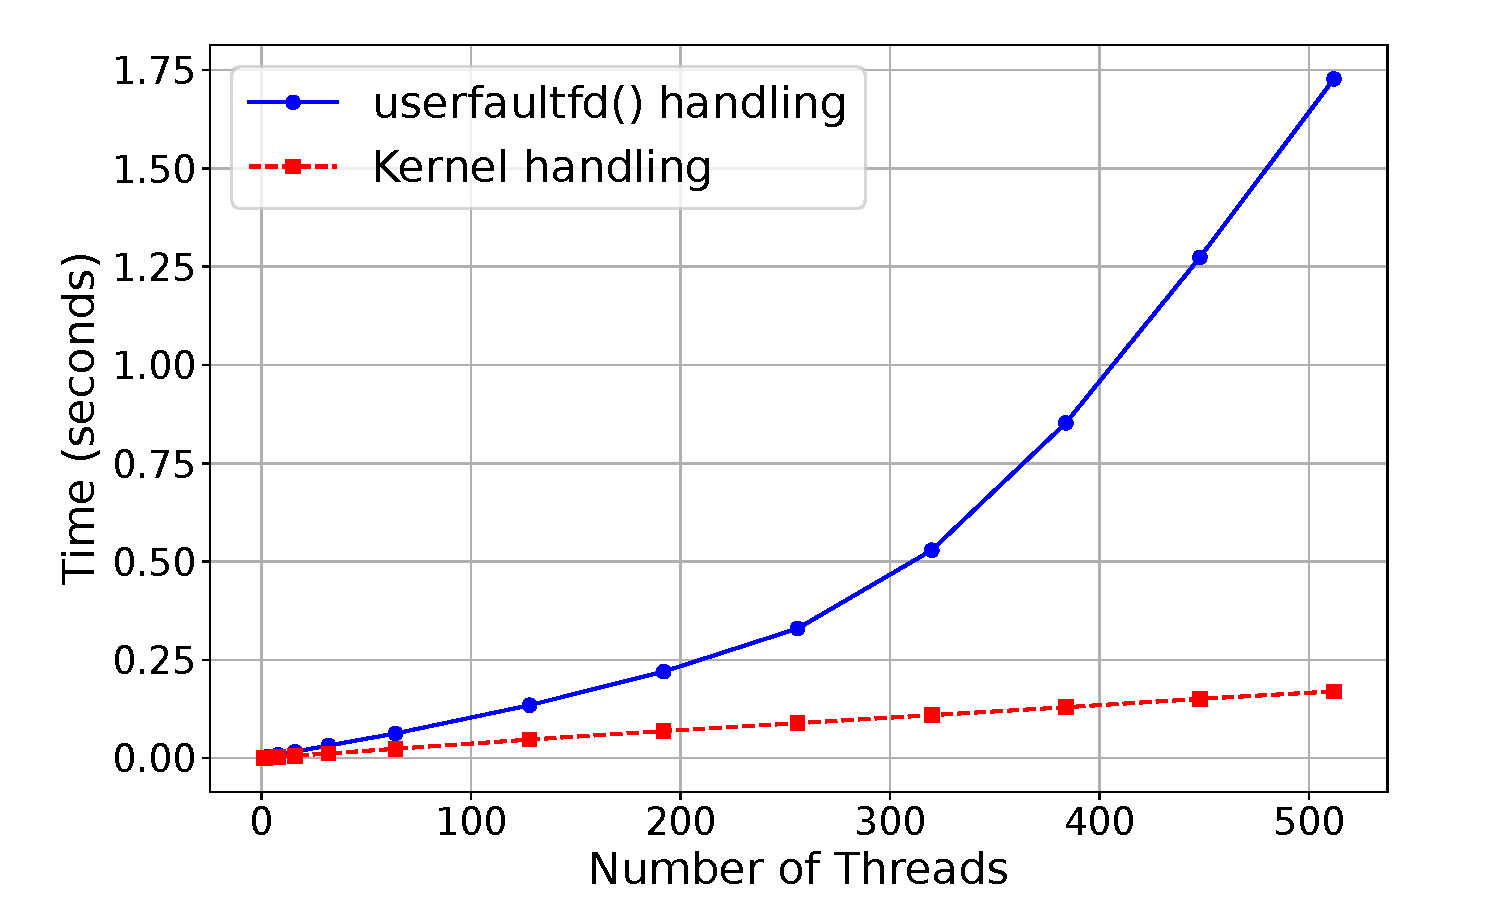
\includegraphics[clip,scale=0.33]{figures/uffd-scalability-motivation.pdf}
    %\vspace{-0.5em}
    \caption{Latency to handle 50 page faults per thread.}
    \label{fig:motivation-scalability}
    %\vspace{-1.0em}
\end{figure}

\textbf{Applicability.} The use of a dedicated fault-handling thread limits which systems can use \texttt{userfaultfd()}.
Specifically, applications that fork may not be able to use \texttt{userfaultfd()}, as forking in a multi-threaded environment only clones the thread that calls \texttt{fork()}, potentially leading to incorrect behavior.
This effectively prevents \texttt{userfaultfd()} from being used in interchangeable libraries, such as the dynamic linker or garbage collectors, which cannot restrict application behavior in such a way.

\textbf{Security.} \texttt{userfaultfd()} has been used in a number of kernel exploits~\cite{uffd-blocking,dirtycred,linux-heap-cve,linux-heap-spray,linux-uaf-cve}, many of which have taken advantage of its ability to indefinitely block kernel execution at a specific point. While mitigations have been proposed and merged~\cite{uffd-blocking}, container runtimes such as Docker have blocked its usage in their default configurations due to these security concerns~\cite{docker-seccomp}, further limiting its applicability.